\chapter{The Revelation Principle and Mechanism Design}

\section{Direct Mechanism and Revelation Principle}

In exploring the optimal way to sell an object to $n$ buyers, we establish a rigorous mathematical framework. Suppose the seller's reservation value for the object is $x_0$, and the buyers' true valuations $X_i$ are drawn independently from a distribution $F_i$.

Any complex selling procedure in reality can be abstracted as a \textit{general mechanism}. This mechanism consists of three mathematical components, denoted as $(\mathcal{B}, \pi, \mu)$:
\begin{itemize}
    \item \textbf{Message Space ($\mathcal{B}$):} The set of messages (or ``bids'') that buyers can submit. For $n$ buyers, the global message space is $\mathcal{B} = \mathcal{B}_1 \times \mathcal{B}_2 \times \dots \times \mathcal{B}_n$.
    \item \textbf{Allocation Rule ($\pi(b)$):} Given a profile of submitted messages $b$, $\pi_i(b)$ determines the probability that buyer $i$ receives the object.
    \item \textbf{Payment Rule ($\mu(b)$):} Given a profile of submitted messages $b$, $\mu_i(b)$ determines the amount that buyer $i$ must pay to the seller.
\end{itemize}
Under this mechanism, suppose the buyers play a game and reach an equilibrium. Each buyer employs an \textit{equilibrium strategy} $\beta_i(x_i)$, which maps their true valuation $x_i$ to an optimal message $b_i$ that maximizes their expected utility.

Analyzing general mechanisms can be mathematically daunting due to the potentially infinite complexity of the message space. To drastically simplify this problem, we introduce the concept of a \textit{direct mechanism}.

In a direct mechanism $([0,1]^n, Q, M)$, the seller simply asks the buyers to report their true valuations directly. Thus, the message space is restricted to the valuation space itself (i.e., $\mathcal{B}_i = [0,1]$). The mechanism's allocation and payment rules are implemented by applying the equilibrium strategies $\beta(x)$ from the original mechanism ``behind the scenes'':
\begin{itemize}
    \item \textbf{Direct Allocation Rule:} $Q_i(x) = \pi_i(\beta(x))$
    \item \textbf{Direct Payment Rule:} $M_i(x) = \mu_i(\beta(x))$
\end{itemize}

\textit{The Revelation Principle} states a profound result: If there exists an equilibrium outcome in some complex general mechanism, we can always construct a corresponding direct mechanism where {truth-telling (reporting true valuations honestly) constitutes an equilibrium for all buyers}. Furthermore, this truth-telling equilibrium yields the exact same allocation probabilities and expected payments as the original mechanism.

This principle is the cornerstone of mechanism design. It greatly simplifies the search for an ``optimal auction'': instead of exhaustively searching through all possible auction formats and bidding rules, the mechanism designer only needs to optimize over the set of direct mechanisms subject to the constraint that buyers are willing to report truthfully (the \textit{incentive compatibility constraint}).
\begin{center}
\begin{tikzpicture}[
    scale=0.85, transform shape, % 这里控制缩放比例，0.85 左右通常比较合适
    node distance=1.5cm and 2.5cm,
    box/.style={draw, rectangle, rounded corners, minimum width=2.8cm, minimum height=1cm, align=center},
    arrow/.style={->, >=stealth, thick},
    label/.style={above, align=center, text width=2.5cm} 
]
    % General Mechanism Flow
    \node[box] (val1) {True Values \\ ($x$)};
    \node[box, right=of val1] (bid) {Submit Message \\ ($b = \beta(x)$)};
    \node[box, right=of bid] (out1) {Allocation \& Payment \\ ($\pi(b), \mu(b)$)};
    
    % 在这里使用 \label 样式，并用 \\ 换行
    \draw[arrow] (val1) -- node[label] {Equilibrium \\ Strategy $\beta$} (bid);
    \draw[arrow] (bid) -- node[label] {General \\ Mechanism} (out1);
    
    % Direct Mechanism Flow
    \node[box, below=1.5cm of val1] (val2) {True Values \\ ($x$)};
    \node[box, right=of val2] (report) {Report Values \\ ($x$)};
    \node[box, right=of report] (out2) {Allocation \& Payment \\ ($Q(x), M(x)$)};
    
    % 这个原文本不长，可以不换行，也可以加换行符作为可选断点
    \draw[arrow] (val2) -- node[label, text width=2cm] {Truth-telling} (report);
    \draw[arrow] (report) -- node[label] {Direct \\ Mechanism} (out2);
    
    % Vertical Equivalence Arrow
    % 将 Complete Equivalence 缩短为 Results Equivalent 并换行
    \draw[<->, >=stealth, dashed, thick, blue!70!black] (out1.south) -- node[label, right, text=blue!70!black, xshift=2pt] {Results \\ Equivalent} (out2.north);
\end{tikzpicture}
\end{center}


\thmp{Revelation Principle}{
  If $\beta$ is an equilibrium of a general mechanism $(\mathcal{B}, \pi, \mu)$, then truth-telling (reporting $x_i$ honestly) is an equilibrium of the corresponding direct mechanism $([0,1]^n, Q, M)$.
}{
  Intuitively, if a buyer found it optimal to play the strategy $\beta(x_i)$ in the original complex mechanism, they will find it optimal to simply report their true type $x_i$ in the direct mechanism, because the direct mechanism automatically plays their optimal strategy $\beta(x_i)$ on their behalf. Any deviation from truth-telling would result in the mechanism executing a sub-optimal strategy for that buyer.
}

\corp{Expected Payment Identity}{
  In any incentive-compatible mechanism with a reserve price $r$, the expected payment $m(x)$ of a bidder with valuation $x \ge r$ is uniquely determined by the allocation rule $G(\cdot)$ and the expected payment of the marginal type $m(r)$. Specifically, it is given by:
  \[
  m(x) = m(r) + \int_r^x y g(y) \d y,
  \]
  where $g(y) = G'(y)$ is the density function associated with the allocation rule.
}{
  Let $U(z | x) = x G(z) - m(z)$ denote the expected utility of a bidder with true valuation $x$ who reports $z$. By the Revelation Principle, we focus on the truth-telling equilibrium where the value function is:
  \[
  V(x) = U(x | x) = \max_z (x G(z) - m(z)).
  \]
  By the Envelope Theorem, the derivative of the value function with respect to $x$ is simply $V'(x) = G(x)$. Integrating this from the reserve price $r$ to $x$ yields:
  \[
  V(x) = V(r) + \int_r^x G(y) \d y.
  \]
  Using the definition $V(x) = x G(x) - m(x)$, we can isolate the expected payment:
  \[
  m(x) = x G(x) - V(r) - \int_r^x G(y) \d y.
  \]
  Applying integration by parts to the term $\int_r^x y g(y) \d y = x G(x) - r G(r) - \int_r^x G(y) \d y$, we can rewrite the payment equation as:
  \[
  m(x) = r G(r) + \int_r^x t g(y) \d y - V(r).
  \]
  Recall that the equilibrium utility for the marginal bidder is $V(r) = r G(r) - m(r)$. Substituting this definition into the equation above immediately yields the desired result:
  \[
  m(x) = m(r) + \int_r^x y g(y) \d y.
  \]
}

\section{Optimal Mechanism Design (Myerson, 1981)}

\subsection{Motivating Example: Monopoly Pricing}

What is the best way to sell an object to $n$ buyers? Let us start with the simplest case: $n = 1$.

Suppose the single buyer's valuation $X$ is drawn from a distribution with cumulative distribution function $F(x)$ and probability density function $f(x)$. The seller wants to post a take-it-or-leave-it price $p$. 

Importantly, let $x_0$ be the \textit{seller's own valuation} (or reservation value) of the object. This represents the utility the seller retains if the transaction fails and they keep the item.

The seller's expected profit $\mathbb{E}[\pi(p)]$ from posting price $p$ consists of two mutually exclusive scenarios:
\begin{itemize}
    \item \textbf{Transaction succeeds (Probability $1-F(p)$):} The buyer's valuation $X \ge p$. The seller collects the payment $p$.
    \item \textbf{Transaction fails (Probability $F(p)$):} The buyer's valuation $X < p$. The seller keeps the object and retains a value of $x_0$.
\end{itemize}

Thus, the expected profit is given by:
\[
\mathbb{E}[\pi(p)] = p \cdot \Pr{X \ge p} + x_0 \cdot \Pr{X < p} = p(1-F(p)) + x_0 F(p)
\]

To find the revenue-maximizing optimal price $p^*$, we take the first derivative of the expected profit with respect to $p$ and set it to zero:
\[
\frac{\d \mathbb{E}[\pi(p)]}{\d p} = (1-F(p)) - pf(p) + x_0 f(p) = 0
\]

By dividing by $f(p)$ and rearranging the terms, we arrive at a profound economic condition:
\[
p^* - \frac{1-F(p^*)}{f(p^*)} = x_0
\]

The expression $p - \frac{1-F(p)}{f(p)}$ is a fundamental concept in mechanism design known as the \textit{virtual value}. The term $\frac{f(p)}{1-F(p)}$ is defined as the \textit{hazard rate} of the valuation distribution. This equation dictates that a revenue-maximizing seller should set the optimal posted price $p^*$ exactly at the point where the buyer's \textit{virtual value} equals the seller's \textit{true valuation} $x_0$. 

\rmk{
  In many standard textbook problems, we assume the object has zero use value to the seller, i.e., $x_0 = 0$. In such cases, the FOC simplifies to $p^* - \frac{1-F(p^*)}{f(p^*)} = 0$.
}

\subsection{Framing Seller's Problem}

By the Revelation Principle, instead of searching through an infinite space of possible game rules and message spaces, the seller \textit{only needs to find the optimal direct mechanism} $(Q, M)$ subject to incentive compatibility (truth-telling) constraints. There is no loss of generality in restricting our attention to direct mechanisms where the message space is simply the type space, $\mathcal{B}_i = [0,1]$. 

The mechanism designer (the seller) optimizes over two functions: the \textit{allocation rule} $Q$ and the \textit{payment rule} $M$:
  \[
  Q: [0,1]^n \to \Delta, \quad M: [0,1]^n \to \mathbb{R}^n,
  \]
  where $\Delta$ is the probability simplex over the $n$ buyers (i.e., $Q_i(x)$ is the probability that buyer $i$ receives the object given the profile of reported valuations $x$).

\defn{Interim Expected Probability of Winning \&\\ Interim Expected Payment}{
  For any bidder $i$, suppose they report their valuation as $z_i$ while all other $n-1$ bidders report truthfully. The \textit{interim expected probability of winning} $q_i(z_i)$ and the \textit{interim expected payment} $m_i(z_i)$ are defined as:
  \[
  \begin{aligned}
    q_i(z_i) & = \int_{[0,1]^{n-1}} Q_i(z_i, x_{-i}) f_{-i}(x_{-i}) \d x_{-i}\\
    m_i(z_i) & = \int_{[0,1]^{n-1}} M_i(z_i, x_{-i}) f_{-i}(x_{-i}) \d x_{-i}
  \end{aligned}
  \]
  where $f_{-i}(x_{-i}) = \prod_{j \neq i} f_j(x_j)$ is the joint density of all other bidders' true valuations.
}

The expected payoff for bidder $i$ with true valuation $x_i$ who reports $z_i$ is therefore:
\[
\pi_i(x_i, z_i) = q_i(z_i) \cdot x_i - m_i(z_i)
\]

To ensure that truth-telling is a Bayesian Nash Equilibrium,\footnote{\textbf{Nash Equilibrium (NE) vs. Bayesian Nash Equilibrium (BNE):} In a traditional NE, players have complete information about the game, including the exact payoffs of all other players. In a mechanism design setting, information is incomplete: a bidder knows their own valuation but only knows the \textit{distribution} of others' valuations. A BNE is the extension of NE to games of incomplete information, where each player's strategy maximizes their \textit{expected} payoff, taking expectations over the possible types of other players based on a common prior distribution.} the mechanism must satisfy the \textit{incentive compatibility constraint}:
\state{Incentive Compatibility Constraint (IC)}{
  A mechanism $(Q, M)$ is \textit{incentive compatible} if the following holds:
  \[
  \pi_i(x_i, z_i) \ge \pi_i(x_i, x_i), \quad \forall i , \quad \forall x_i \in [0,1],\quad \forall z_i \in [0,1].
  \]
}

If the IC constraint is satisfied, every bidder will tell the truth. In this case, we can express the equilibrium payoff of bidder $i$ as a function of their true type $x_i$:
\[
u_i(x_i) \equiv \pi_i(x_i, x_i) = \max_{z_i} \left\{ q_i(z_i) \cdot x_i - m_i(z_i) \right\}
\]

\clmp{Properties of the IC Mechanism}{
  From the definition of the equilibrium payoff function $u_i(x_i)$,
  \[
  u_i(x_i) \equiv \pi_i(x_i, x_i) = \max_{z_i} \left\{ q_i(z_i) \cdot x_i - m_i(z_i) \right\},
  \] we immediately obtain three fundamental results:
  \begin{enumerate}
      \item $u_i(x_i)$ is a convex function of $x_i$.
      \item $u_i'(x_i) = q_i(x_i)$ almost everywhere.
      \item $q_i(x_i)$ is non-decreasing in $x_i$.
  \end{enumerate}
}{
  \begin{itemize}
      \item \textbf{Convexity:} The value function $u_i(x_i)$ is defined as the upper envelope (the point-wise maximum) of a family of functions in $x_i$. Since $q_i(z_i)x_i - m_i(z_i)$ is an affine (linear) function of $x_i$, their upper envelope is globally convex.\footnote{\textbf{Linear vs. Affine:} Strictly speaking, a \textit{linear} function must pass through the origin ($f(x) = ax$), whereas an \textit{affine} function is a linear function plus a constant translation ($f(x) = ax + b$). Sometimes economists sometimes use the terms interchangeably.}
      \item \textbf{Envelope Theorem:} By the Envelope Theorem, the total derivative of the maximized value function with respect to the parameter $x_i$ equals the partial derivative of the objective function evaluated at the optimal choice ($z_i = x_i$). Thus, $u_i'(x_i) = q_i(x_i)$.
      \item \textbf{Monotonicity:} Because $q_i(x_i) = u_i(x_i)$ and thus $q_i'(x_i) = u_i'(x_i)$, and $u_i$ is convex ($u_i''(x_i) \ge 0$), $q_i(x_i)$ is naturally non-decreasing in $x_i$.
  \end{itemize}
}

\propp{Allocation Rule Uniquely Determines Payment Rule}{
  In any incentive-compatible (IC) and individually rational (IR) mechanism designed by a profit-maximizing seller, the equilibrium expected payoff $u_i(x_i)$ and the expected payment $m_i(x_i)$ for any bidder $i$ are completely and uniquely determined by the allocation rule $Q$. Specifically, the lowest type extracts zero surplus ($u_i(0) = 0$), yielding the exact payoff function:
  $$u_i(x_i) = \int_0^{x_i} q_i(t) \d t$$
}{
  Since $u_i'(x_i) = q_i(x_i)$, we can express the payoff function as an integral of the interim winning probability:
  $$u_i(x_i) = u_i(0) + \int_0^{x_i} q_i(t) \d t$$
  
  This implies that once the allocation rule $Q$ (and thus the interim probability $q_i$) is fixed, the equilibrium payoff function $u_i$ is entirely pinned down up to a constant $u_i(0)$. Loosely speaking, the IC constraint determines the \textit{shape} of the payoff function. Consequently, the shape of the expected payment $m_i(x_i) = q_i(x_i)x_i - u_i(x_i)$ is also uniquely determined by $Q$.

  Furthermore, to maximize revenue, the seller should extract as much surplus as possible without violating the \textit{individual rationality constraint}: 
  
  \state{Individual Rationality Constraint (IR)}{
    A mechanism $(Q, M)$ is \textit{individually rational} if the following holds:  
    $$u_i(x_i) \ge 0, \quad \forall i.$$
  }

  Since $u_i(x_i)$ is non-decreasing, the IR constraint is satisfied everywhere if and only if $u_i(0) \ge 0$. Note that by definition, $u_i(0) = q_i(0)\cdot 0 - m_i(0) = -m_i(0)$, so:
  $$u_i(0) \ge 0 \implies m_i(0) \le 0.$$
  
  Because the seller is a profit-maximizer, $m_i(0)\le 0$ immediately implies they will set $m_i(0) = 0$, which means $u_i(0) = 0$. Thus:
  $$u_i(x_i) = \int_0^{x_i} q_i(t) \d t.$$
  
  That is, the IR constraint further pins down the constant term in the payoff function, leaving \textit{zero degrees of freedom} for the payoff function (and thus the payment rule) once the allocation rule $Q$ is fixed.
}

The seller's ultimate problem is to maximize total expected revenue:
\[
\max_{Q, M} \sum_{i=1}^n \int_0^1 m_i(x_i) f_i(x_i) \d x_i
\]

Substitute the expected payment identity $m_i(x_i) = q_i(x_i)x_i - \int_0^{x_i} q_i(t) \d t$ into the integral for bidder $i$:
\[
\int_0^1 m_i(x_i) f_i(x_i) \d x_i = \int_0^1 q_i(x_i)x_i f_i(x_i) \d x_i - \int_0^1 \left( \int_0^{x_i} q_i(t) \d t \right) f_i(x_i) \d x_i
\]

We swap the order of integration for the second term (visual proof below):
\[
\int_0^1 \int_0^{x_i} q_i(t) \d t f_i(x_i) \d x_i = \int_0^1 \int_{t}^1 f_i(x_i) \d x_i \, q_i(t) \d t = \int_0^1 (1 - F_i(x_i)) q_i(x_i) \d x_i
\]
\begin{center}
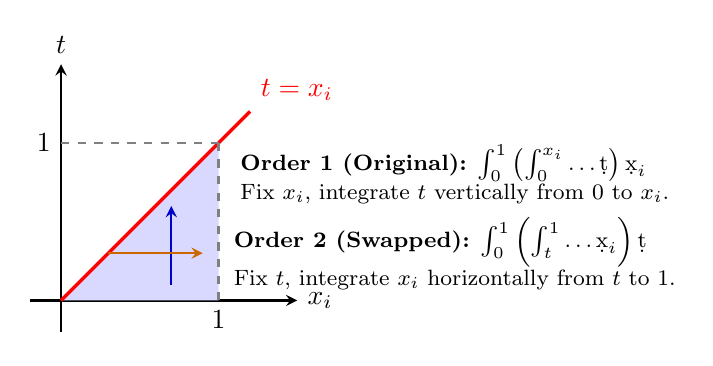
\begin{tikzpicture}[scale=2, thick, every node/.style={font=\sffamily}]
  % Axes
  \draw[->, >=stealth] (-0.2, 0) -- (1.5, 0) node[right] {$x_i$};
  \draw[->, >=stealth] (0, -0.2) -- (0, 1.5) node[above] {$t$};
  
  % Region of integration
  \fill[blue!15] (0,0) -- (1,0) -- (1,1) -- cycle;
  
  % The line t = x_i
  \draw[red, very thick] (0,0) -- (1.2,1.2) node[above right] {$t = x_i$};
  
  % Bounding box
  \draw[dashed, gray] (1,0) node[below, text=black] {$1$} -- (1,1);
  \draw[dashed, gray] (0,1) node[left, text=black] {$1$} -- (1,1);
  
  % Node explaining the two ways to integrate
  \node[align=left, font=\footnotesize, text=black] at (2.5, 0.8) {
    \textbf{Order 1 (Original):} $\int_0^1 \left( \int_0^{x_i} \dots \d t \right) \d x_i$ \\
    Fix $x_i$, integrate $t$ vertically from $0$ to $x_i$.
  };
  \node[align=left, font=\footnotesize, text=black] at (2.5, 0.3) {
    \textbf{Order 2 (Swapped):} $\int_0^1 \left( \int_t^1 \dots \d x_i \right) \d t$ \\
    Fix $t$, integrate $x_i$ horizontally from $t$ to $1$.
  };
  
  % Arrows to show integration directions
  \draw[->, >=stealth, blue!80!black] (0.7, 0.1) -- (0.7, 0.6); % Vertical
  \draw[->, >=stealth, orange!80!black] (0.3, 0.3) -- (0.9, 0.3); % Horizontal
\end{tikzpicture}
\end{center}

Substituting this back into the revenue equation gives us the expected revenue purely as a function of the allocation rule:
\[
\int_0^1 m_i(x_i) f_i(x_i) \d x_i = \int_0^1 \left[ x_i - \frac{1 - F_i(x_i)}{f_i(x_i)} \right] q_i(x_i) f_i(x_i) \d x_i
\]
We define the bracketed term as the \textit{virtual value}:
\defn{Virtual Value}{
  The \textit{virtual value} of a bidder with true type $x_i$, denoted by $\phi_i(x_i)$, is defined as
  \[
  \phi_i(x_i) = x_i - \frac{1 - F_i(x_i)}{f_i(x_i)}.
  \]
}

\textbf{Why?} To understand the logical leap to "money", we must look at the mechanics of the Incentive Compatibility (IC) constraint: $u_i(x_i) = \int_0^{x_i} q_i(t)\d t$. 
  
  Suppose the seller decides to increase the allocation probability $q_i(x)$ for a specific type $x$. Because the expected payoff $u_i$ is the integral of $q_i$ from $0$ up to the true type, increasing $q_i(x)$ does not just increase the payoff for type $x$—it automatically increases the payoff for \textit{every single type strictly greater than $x$}! 
  
  If the seller makes it attractive for type $x$ to win the object, mimicking type $x$ suddenly becomes very tempting for everyone with a higher valuation. To prevent all higher types from lying and claiming to be type $x$ to get a cheaper price, the seller is forced to "bribe" them by leaving more surplus (money) on the table. 
  
  How many higher types are there? The probability mass of bidders with a valuation $> x$ is exactly $1 - F_i(x)$. Therefore, $1 - F_i(x)$ represents the total volume of "bribes" (information rent) the seller must pay out to the upper tail of the distribution. Dividing this by the local density $f_i(x)$ simply normalizes this total cost into a \textit{marginal} cost evaluated at type $x$. 
  
  Thus, $\frac{1-F_i(x_i)}{f_i(x_i)}$ is exactly the expected dollar amount of surplus the mechanism must concede \textit{locally} at type $x_i$: allocating to $x_i$ forces the seller to surrender rent to the $1-F_i(x_i)$ mass of people above them!

\rmkb[Understanding the Information Rent]{
  The virtual value $\phi_i(x_i)$ is strictly less than the true valuation $x_i$. The subtracted term, $\frac{1-F_i(x_i)}{f_i(x_i)}$ (the inverse hazard rate), represents the \textit{information rent}. This is because of the IC constraint: If the seller allocates the object to a bidder with valuation $x_i$, they cannot simply charge them $x_i$. To prevent all types strictly higher than $x_i$ from lying and mimicking type $x_i$ to get a cheaper price, the seller must leave some surplus (rent) on the table for those higher types.

  By the Envelope Theorem, a bidder of type $x_i$ earns a payoff of $u_i(x_i) = \int_0^{x_i} q_i(t)\d t$. When we take the expectation of this payoff across all possible types, the mathematical result is $\mathbb{E}[u_i] = \mathbb{E}\left[q_i(x_i) \frac{1-F_i(x_i)}{f_i(x_i)}\right]$. Thus, $\frac{1-F_i(x_i)}{f_i(x_i)}$ is exactly the expected dollar amount of surplus (information rent) the mechanism must concede \textit{locally} at type $x_i$ to ensure all higher types truthfully reveal themselves.
  
  Therefore, $\phi_i(x_i)$ is the \textit{actual marginal revenue} the seller extracts when allocating the object to a bidder with value $x_i$.
}

Recall that by definition, the interim allocation probability is the expected value of the ex-post allocation rule over all other bidders' types:
\[
q_i(x_i) = \int_{[0,1]^{n-1}} Q_i(x_i, x_{-i}) f_{-i}(x_{-i}) \d x_{-i}
\]

By expanding $q_i(x_i)$ back into the joint integral over all $n$ bidders, the seller's optimization problem simplifies remarkably to maximizing the expected virtual surplus:
\[
\max_{Q} \int_{[0,1]^n} \left[ \sum_{i=1}^n \phi_i(x_i) Q_i(x) \right] f(x) \d x
\]
subject to the physical constraints that $Q_i(x) \in [0,1]$, $\sum Q_i(x) \le 1$, and the IC monotonicity constraint that $q_i(\cdot)$ is non-decreasing.

\asm{Regularity Condition on $\phi_i$}{
  The virtual value $\phi_i(x_i)$ is strictly increasing in $x_i$.
}

\rmkb[Why Regularity Guarantees Monotonicity]{
  To understand why this condition is critical, recall that the seller's objective is to maximize the expected virtual surplus. For any given profile of reported types $x$, the seller wants to choose an allocation rule $q(x)$ to maximize:
  $$\max_{q} \sum_{i=1}^n q_i(x) \phi_i(x_i)$$
  subject to the feasibility constraint $\sum q_i(x) \le 1$.

  Ignoring the IC constraint for a moment, the unconstrained optimal way to maximize this sum is simply to allocate the object to the bidder with the highest strictly positive virtual value. That is, $q_i(x) = 1$ if $\phi_i(x_i) > \max_{j \neq i} \phi_j(x_j)$ and $\phi_i(x_i) > 0$.

  Recall from the Envelope Theorem that for a mechanism to be Incentive Compatible (IC), the interim allocation probability $q_i(x_i)$ must be non-decreasing in $x_i$.

  If the Regularity Condition holds (i.e., $\phi_i$ is strictly increasing), then a higher true type $x_i$ directly translates to a strictly higher virtual value $\phi_i(x_i)$. A higher virtual value makes it strictly more likely that bidder $i$ outbids all competitors and clears the seller's reserve price. Therefore, the allocation probability $q_i(x_i)$ naturally goes up as $x_i$ goes up. 
  
  In short, the regularity condition ensures that the greedy, unconstrained pointwise maximization algorithm \textit{automatically} satisfies the global IC monotonicity constraint! (If regularity fails and $\phi_i$ decreases in some regions, higher types might be assigned lower probabilities, violating IC.)
}

This regularity condition eensures that pointwise maximization naturally satisfies the monotonicity constraint of $q_i$. 

\prop{Optimal Allocation Rule and Reserve Prices}{
  Under the regularity assumption, we can solve the integral via \textit{pointwise maximization}. For any realized profile of valuations $x = (x_1, \dots, x_n)$, the seller should simply examine the virtual values and assign the object to the bidder with the highest virtual value, provided it is non-negative.

  Mathematically, the optimal allocation rule is:
  \[
  Q_i^*(x) = 
  \begin{cases} 
  1 & \text{if } \phi_i(x_i) = \max_j \phi_j(x_j) \text{ and } \phi_i(x_i) \ge 0 \\
  0 & \text{otherwise}
  \end{cases}
  \]
}

From this, the seller can define an optimal reserve price for each bidder as follows:
\defn{Individual Reserve Price}{
  The optimal reserve price $r_i^*$ for bidder $i$ is exactly the root of their virtual value function:
  \[
  \phi_i(r_i^*) = 0 \implies r_i^* - \frac{1 - F_i(r_i^*)}{f_i(r_i^*)} = 0
  \]
}
Notably, to maximize revenue, the seller does \textit{not} necessarily allocate the object to the person with the highest true value, but to the person with the highest \textit{virtual value}. Furthermore, if no bidder's virtual value exceeds zero (i.e., everyone's valuation is below their respective $r_i^*$), the seller optimally retains the object to avoid paying excessive information rents. From this perspective, the optimal mechanism is to allocate the object to the buyer with the highest valuation \textit{strictly above their respective reserve price}.

\subsection{The Monopoly Pricing Isomorphism: What is Virtual Value?}

While the derivation of the optimal mechanism using the Envelope Theorem and integration by parts is mathematically rigorous, the economic intuition behind the \textit{virtual valuation} can be beautifully illuminated by a simple parallel: \textit{Standard Monopoly Pricing}.

Imagine a monopolist selling a single object to a market of buyers whose valuations are distributed according to $F(\cdot)$ with density $f(\cdot)$. 

\clmp{Virtual Valuation is Marginal Revenue}{
  If we view the probability of sale as the ``quantity" demanded, the virtual valuation $\psi(p)$ is exactly the monopolist's marginal revenue evaluated at price $p$.
}{
  Let $p$ be the price set by the monopolist. A buyer will purchase the object if their valuation is greater than or equal to $p$. Thus, the quantity demanded $q$ at price $p$ is exactly the survival function:
  $$q(p) = 1 - F(p)$$
  
  To find the marginal revenue, we first need the inverse demand curve $P(q)$. By inverting the demand function, we get:
  $$P(q) = F^{-1}(1-q)$$
  
  The monopolist's total revenue $R(q)$ as a function of quantity is price times quantity:
  $$R(q) = q \cdot P(q) = q \cdot F^{-1}(1-q)$$
  
  Now, we differentiate $R(q)$ with respect to $q$ to find the $MR$:
  $$
  \begin{aligned}
    MR(q) & = \frac{\d R(q)}{\d q} \\
    & = F^{-1}(1-q) + q \left[ \frac{1}{f(F^{-1}(1-q))} \cdot (-1) \right]\\
  & = F^{-1}(1-q) - \frac{q}{f(F^{-1}(1-q))}
  \end{aligned}
  $$
  
  Finally, we substitute the original price variable $p = F^{-1}(1-q)$ and quantity $q = 1 - F(p)$ back into the $MR$ equation to express marginal revenue as a function of price:
  $$MR(p) = p - \frac{1 - F(p)}{f(p)}$$
  
  This expression is exactly the definition of the \textit{virtual valuation}
}

This profound mathematical equivalence means we can analyze optimal auction mechanisms using the familiar geometric tools of intermediate microeconomics. The optimal mechanism simply allocates the good to the buyer with the highest $MR$, provided $MR \ge MC$ (where $MC$ could be the seller's own value $c$).

\begin{center}
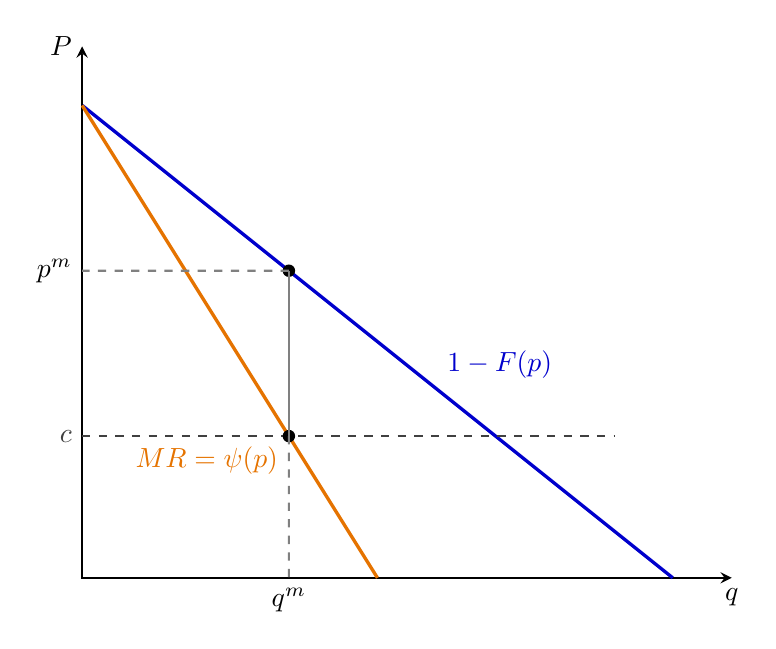
\begin{tikzpicture}[scale=1.5, thick, every node/.style={font=\sffamily}]
  % Axes
  \draw[<->, >=stealth] (0, 4.5) node[left] {$P$} -- (0, 0) -- (5.5, 0) node[below] {$q$};
  
  % Define curves
  % Demand curve: p = 4 - 0.8q
  \draw[blue!80!black, very thick] (0, 4) -- (5, 0) node[pos=0.6, above right] {$1 - F(p)$};
  
  % MR curve: MR = 4 - 1.6q
  \draw[orange!90!black, very thick] (0, 4) -- (2.5, 0) node[pos=0.7, below left] {$MR = \psi(p)$};
  
  % MC curve: Horizontal line at c = 1.2
  \draw[dashed, darkgray, thick] (0, 1.2) node[left] {$c$} -- (4.5, 1.2);
  
  % Intersection of MR and MC (Optimal Quantity q^m)
  % 4 - 1.6q = 1.2 => 1.6q = 2.8 => q = 1.75
  \coordinate (Opt) at (1.75, 1.2);
  \fill[black] (Opt) circle (1.5pt);
  
  % Dashed line down to q^m
  \draw[dashed, gray, thick] (Opt) -- (1.75, 0) node[below, text=black] {$q^m$};
  
  % Point on Demand curve (Monopoly Price p^m)
  % p = 4 - 0.8(1.75) = 4 - 1.4 = 2.6
  \coordinate (Pm_point) at (1.75, 2.6);
  \fill[black] (Pm_point) circle (1.5pt);
  \draw[solid, gray, thick] (Opt) -- (Pm_point);
  
  % Dashed line left to p^m
  \draw[dashed, gray, thick] (Pm_point) -- (0, 2.6) node[left, text=black] {$p^m$};
  
  % Optional: highlight the rectangles for revenue / information rent intuitively
  % \fill[blue!10, opacity=0.5] (0,0) rectangle (1.75, 2.6);
  
\end{tikzpicture}
\end{center}

\rmkb[Information Rent is the Inframarginal Loss]{
  Why does the inverse hazard rate $\frac{1-F(p)}{f(p)}$ appear in both mechanism design and standard monopoly pricing? 
  
  In intermediate microeconomics, to sell one additional unit (i.e., to induce a buyer with a slightly lower valuation to buy), the monopolist must lower the price. However, because price discrimination is impossible, the monopolist must lower the price not just for this marginal buyer, but for \textit{all inframarginal buyers} who would have been willing to pay a higher price. This loss in revenue on the inframarginal units drives a wedge between the price $p$ and the marginal revenue $MR$.
  
  In mechanism design, this exact same dynamic is what we call the \textbf{Information Rent}. To convince a high-type buyer to reveal their true valuation rather than mimicking a lower type, the mechanism designer must leave them some surplus. The "loss of revenue on inframarginal buyers" in the monopoly model is mathematically identical to the "information rent paid to higher types" to satisfy the Incentive Compatibility (IC) constraint!
}

